%! Author = dayan3847
%! Date = 4/30/23

% Preamble
\documentclass[11pt]{article}

% Packages
\usepackage{amsmath}
\usepackage{hyperref}
\usepackage{amssymb}
\usepackage{tikz}

\usepackage{multicol}
\usepackage{biblatex}
\usepackage{cancel}
\usepackage{amsfonts}


\title{Rango de $r$}
\author{Dayan Bravo Fraga}
\date{Abril 2023}

% Document
\begin{document}
    \maketitle


    \section{Interrogante}\label{sec:question_mark}

    ¿Cuál es el rango de $r$ en la transformación de Hough para rectas?


    \section{Desmotración}\label{sec:demonstration}

    Tenemos la siguiente ecuación:

    \begin{equation}
        \label{eq:1}
        r = x \cos(\theta) + y \sin(\theta)
    \end{equation}

    El dominio de $\theta$ es:

    \begin{equation}
        \label{eq:2}
        \theta \in [0, \pi]
    \end{equation}

    Si tenemos que $m$ y $n$ son el ancho y alto de la imagen respectivamente (cantidad de pixeles), entonces:

    \begin{equation}
        \label{eq:3}
        x \in \mathbb{N}, 1 \leq x \leq m-1, m > 0
    \end{equation}

    \begin{equation}
        \label{eq:4}
        y \in \mathbb{N}, 1 \leq y \leq n-1, n > 0
    \end{equation}

    Ahora graficaremos las funciones $\cos(\theta)$ y $\sin(\theta)$ para $\theta \in [0, \pi]$:

    \begin{multicols}{2}
        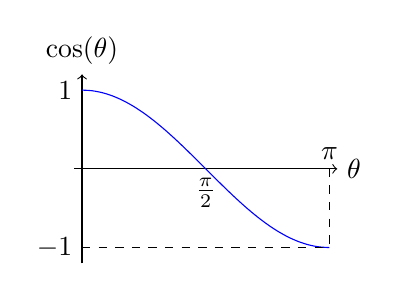
\begin{tikzpicture}
            \draw[->] (-.1,0) -- (pi+.1,0) node[right] {$\theta$};
            \draw[->] (0,-1.2) -- (0,1.2) node[above] {$\cos(\theta)$};
            \draw[
                domain=0:pi,
                smooth,
                variable=\theta,
                blue
            ] plot ({\theta},{cos(\theta r)});
            \draw[dashed] (pi,0) -- (pi,-1);
            \draw[dashed] (0,-1) -- (pi,-1);
            \draw node at (pi/2,0) [below] {$\frac{\pi}{2}$};
            \draw node at (pi,0) [above] {$\pi$};
            \draw node at (0,1) [left] {$1$};
            \draw node at (0,-1) [left] {$-1$};
        \end{tikzpicture}
        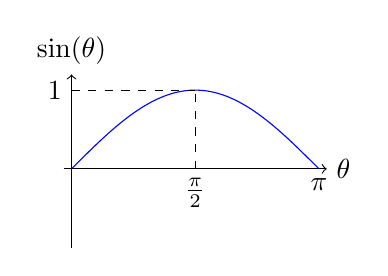
\begin{tikzpicture}
            \draw[->] (-.1,0) -- (pi+.1,0) node[right] {$\theta$};
            \draw[->] (0,-1) -- (0,1.2) node[above] {$\sin(\theta)$};
            \draw[
                domain=0:pi,
                smooth,
                variable=\theta,
                blue
            ] plot ({\theta},{sin(\theta r)});
            \draw[dashed] (pi/2,0) -- (pi/2,1);
            \draw[dashed] (0,1) -- (pi/2,1);
            \draw node at (pi/2,0) [below] {$\frac{\pi}{2}$};
            \draw node at (pi,0) [below] {$\pi$};
            \draw node at (0,1) [left] {$1$};
        \end{tikzpicture}
    \end{multicols}
    De las gráficas podemos deducir que, si sumamos ambas funciones ($\cos(\theta)$ y $\sin(\theta)$):
    \begin{itemize}
        \item El valor máximo es en $ 0 < \theta < \pi/2$
        \item El valor mínimo es en $\theta = \pi$
    \end{itemize}

    Ahora graficaremos la Función $r = x \cos(\theta) + y \sin(\theta)$,
    en $\theta \in [0, \pi]$,
    para $x = 1$ y $y = 1$:

    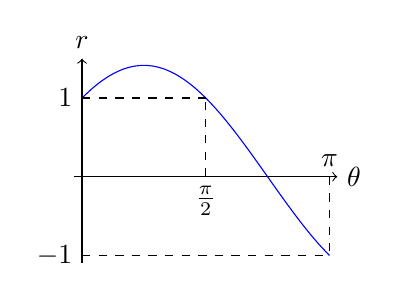
\begin{tikzpicture}
        \draw[->] (-.1,0) -- (pi+.1,0) node[right] {$\theta$};
        \draw[->] (0,-1.1) -- (0,1.5) node[above] {$r$};
        \draw[
            domain=0:pi,
            smooth,
            variable=\theta,
            blue
        ] plot ({\theta},{cos(\theta r) + sin(\theta r)});
        \draw[dashed] (pi,0) -- (pi,-1);
        \draw[dashed] (0,-1) -- (pi,-1);
        \draw[dashed] (pi/2,0) -- (pi/2,1);
        \draw[dashed] (0,1) -- (pi/2,1);
        \draw node at (pi/2,0) [below] {$\frac{\pi}{2}$};
        \draw node at (pi,0) [above] {$\pi$};
        \draw node at (0,1) [left] {$1$};
        \draw node at (0,-1) [left] {$-1$};
    \end{tikzpicture}

    Como podemos observar, se confirma lo que habíamos deducido anteriormente.

    \subsection{Valor mínimo de $r$}\label{subsec:min_r}

    En caso del valor mínimo de $r$, se da cuando $\theta = \pi$,
    entonces, si sustituimos en la ecuación~\ref{eq:1}:

    \begin{gather*}
        r = x \cos(\pi) + y \sin(\pi)\\
        r = x \cancel{\cos(\pi)}^{-1} + \cancel{y \sin(\pi)}^0\\
        r = -x
    \end{gather*}

    Como $x \in [0, m-1]$, entonces $-x \in [-m+1, 0]$.

    Entonces, el valor mínimo de $r$ es $-m+1$.

    \subsection{Valor máximo de $r$}\label{subsec:max_r}

    Para calcular el valor máximo de $r$ vamos a derivar la ecuación~\ref{eq:1},
    para $x = 1$ y $y = 1$:

    \begin{gather*}
        r = \cos(\theta) + \sin(\theta)\\
        \frac{dr}{d\theta} = - \sin(\theta) + \cos(\theta)
    \end{gather*}

    Podemos graficar esta nueva funcion para analizar su comportamiento:

    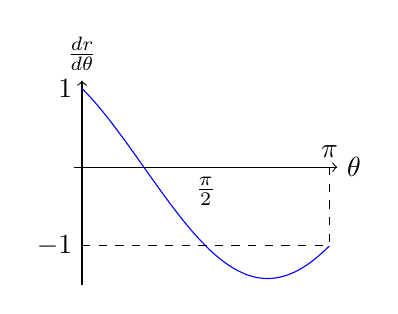
\begin{tikzpicture}
        \draw[->] (-.1,0) -- (pi+.1,0) node[right] {$\theta$};
        \draw[->] (0,-1.5) -- (0,1.1) node[above] {$\frac{dr}{d\theta}$};
        \draw[
            domain=0:pi,
            smooth,
            variable=\theta,
            blue
        ] plot ({\theta},{- sin(\theta r) + cos(\theta r)});
        \draw[dashed] (pi,0) -- (pi,-1);
        \draw[dashed] (0,-1) -- (pi,-1);
        \draw node at (pi/2,0) [below] {$\frac{\pi}{2}$};
        \draw node at (pi,0) [above] {$\pi$};
        \draw node at (0,-1) [left] {$-1$};
        \draw node at (0,1) [left] {$1$};
    \end{tikzpicture}

    Debemos calcular el $cero$ de la función, para ello, igualamos a cero la derivada:

    \begin{gather*}
        - \sin(\theta) + \cos(\theta) = 0\\
        \sin(\theta) = \cos(\theta)\\
        \frac{\sin(\theta)}{\cos(\theta)} = 1\\
        \tan(\theta) = 1\\
        \theta = \frac{\pi}{4}
    \end{gather*}

    Ahora podemos sustituir $\theta = \frac{\pi}{4}$ en la ecuación~\ref{eq:1}:

    \begin{gather*}
        r = x \cos(\frac{\pi}{4}) + y \sin(\frac{\pi}{4})\\
        r = \frac{x \sqrt{2}}{2} + \frac{y \sqrt{2}}{2}\\
        r = \frac{\sqrt{2}}{2} (x + y)
    \end{gather*}

    Lamentablemente este no es el valor máximo absoluto de $r$, es el valor máximo de $r$ cuando $x = 1$ y $y = 1$,
    aunque se podría generalizar a cuando $x = y$.

    Como es una suma de funciones, su valor máximo pudiera ser estimado con los valores máximos de cada función.

    \begin{gather*}
        r = x \cos(\theta) + y \sin(\theta)\\
        r = x \cancel{\cos(\theta)}^1 + y \cancel{\sin(\theta)}^1\\
        r = x + y
    \end{gather*}

    Note que $r$ siempre será menor que este valor, ya que no existe ningún valor de $\theta$ que haga que $\cos(\theta)$ y $\sin(\theta)$ sean $1$ al mismo tiempo.

    Como $x \in [0, m-1]$ y $y \in [0, n-1]$, entonces $x + y \in [0, m + n - 2]$.

    Entonces, el valor máximo de $r$ es $m + n - 2$.

    \fbox{
        \parbox{\textwidth}{
            Nota:

            Si la $x$ es muy grande con respecto a $y$, el valor máximo de $r$ se acercará a $x$,
            por el ángulo $0$, donde el $\cos(\theta) = 1$

            De forma similar, si $y$ es muy grande con respecto a $x$, el valor máximo de $r$ se acercará a $y$,
            por el ángulo $\pi/2$, donde el $\sin(\theta) = 1$
        }
    }

    \subsection{Rango de $r$}\label{subsec:rango_r}

    El rango de $r$ es $ r \in [-m+1, m + n - 2)$.


\end{document}